\chapter{Evaluation}
In this chapter, we evaluate \textsf{Flycatcher}, by using it to generate unit tests for a chosen set of programs. First, we present a summary of the parameters available to \textsf{Flycatcher} users. We then explain our rationale and constraints in choosing the benchmark programs. Next, we describe the experiments and present the results for each program before discussing the results obtained.

\section{\textsf{\mdseries{Flycatcher}} parameters}
In order to understand the parameters used in the experiments carried out in this section, we give a summary of the parameters available to \textsf{Flycatcher} users. Those options can be seen in the screenshot of \textsf{Flycatcher}'s usage information in Figure \ref{params}. We then consider the parameters that can impact our experiments' results, and specify what value they will take.

\begin{figure}
\hspace*{-2cm}
\centering
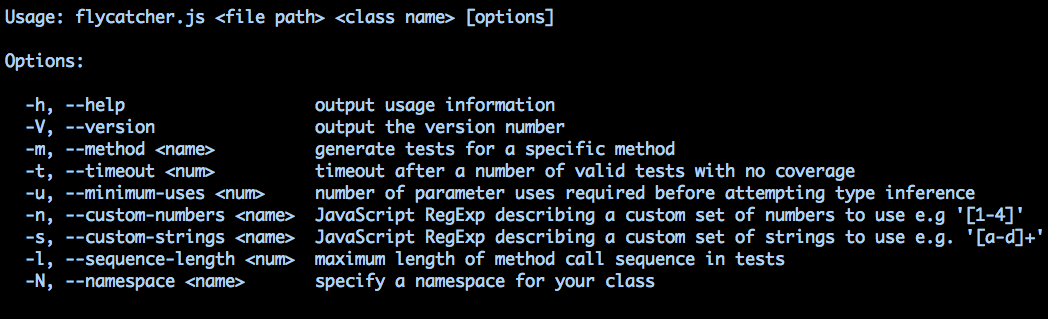
\includegraphics[scale=0.45]{./components/chapter7/params.png}
\caption{\textsf{Flycatcher} parameters}
\label{params}
\end{figure}

\subsection{Specifying the MUT}
Since the collection of information about parameter types happens early on in the test generation process, when testing a whole class, methods tested later benefit from the information collected for the earlier methods. As a result, the time necessary to achieve desired coverage will be much shorter for the later methods, when the test generation process happens for an entire class, as does by default. So that we can carry out effective comparisons and evaluation, we therefore test specific methods of our benchmark classes, such that the type inference stage is taken into account every time.

\subsection{Choosing a timeout}
\textsf{Flycatcher}'s timeout mechanism does not consist of a fixed deadline but a more telling measure, which adapts to the program under test: the number of \emph{valid}\footnote{tests for which we have already inferred types for all parameters involved} tests that are generated without achieving any coverage. This number indicates that the part of the code that remains to be covered is either unreachable or deeply nested. However, in the event that it is the former, a certain termination criterion needs to be decided upon. For both experiments carried out in this section, the timeout chosen was \emph{5000 tests}.

\subsection{Parameter use before inference}
A key feature of \textsf{Flycatcher} is the ability to let the user decide with how much confidence the type of parameters should be inferred. The measure of confidence in inferring a type for a parameter lies in the number of times that parameter has been used in a test. The more the parameter has been used, the more data will have been collected about its type and the stronger the type inference. \underline{The first experiment will consist in varying this parameter} to observe its effect. In the second experiment we will fix it to \texttt{10}.

\subsection{Custom data generators}
So that the random input strings and numbers that are generated by \textsf{Flycatcher} for the unit tests are \emph{appropriate} for the program under test, custom generators can be specified for each. They are specified by a string which represents a regular expression that conforms to the JavaScript RegExp syntax. When the benchmark tests require custom data generators, these will be specified when we discuss the experiments themselves.

\subsection{Setting the maximum length for tests}
When generating object-oriented tests, once the object under test has been initialised, a certain number of methods are called on that object in an attempt to modify its state before calling the MUT. The idea is that this improves code coverage of the MUT. However, as the length of the method call sequence in tests varies, so does the time it takes to achieve full coverage for a MUT. Increasing the length of method call sequences initially speeds up the test generation process, but the tests become too big, the overall process slows down. In trying to find the optimal value for the length of tests for each program, \underline{the second experiment will consist in varying this parameter}.

\section{Choosing the benchmark suite}
In choosing a suite of programs for evaluating \textsf{Flycatcher} we had the following objectives in mind:

\begin{itemize}
   \item Demonstrate \textsf{Flycatcher}'s ability to infer primitive types
   \item Demonstrate \textsf{Flycatcher}'s ability to infer used-defined types
   \item Demonstrate that \textsf{Flycatcher} works for MUT of various size, complexity and number of parameters
   \item Demonstrate \textsf{Flycatcher}'s ability to achieve good (sometimes full) coverage of a MUT in a reasonable time
\end{itemize}

However the constraints imposed to us by the current limitations of the \textsf{Flycatcher} application, made finding benchmark tests difficult. The constraints are the following:

\begin{itemize}
   \item \textsf{Flycatcher} does not handle the inference of \texttt{Array} parameters
   \item \textsf{Flycatcher} does not handle the inference of \texttt{Function} parameters
\end{itemize}

The reason why these constraints made it difficult to find benchmark programs is that array parameters are commonplace and because functions are first-class objects in JavaScript, they frequently occur as parameters too. This also indirectly imposed a restriction on the size of the benchmark programs --- most significant libraries and modules make use of either arrays or functions as parameters at some point. Nevertheless, we were still able to evaluate whether we accomplished what we initially set out to do: build an automatic test generator for a comprehensive \emph{subset} of the JavaScript language.

With these objectives and constraints in mind, the list of methods in Table \ref{benchmarktests} was put together. Some of the programs are custom, many were found using \textsf{Node.js}'s open-source module registry \textsf{npm} and others were taken from the Google V8 performance benchmark suite.

% \begin{table}[h]
% \centering
% \begin{tabular}{|l|l|c|}
% \hline
% \textbf{Class} & \textbf{Method} & \textbf{LOC} \\
% \hline
% \texttt{Triangle} & & \\
%            & \textit{getType} & 38      \\
% \hline
% \texttt{LinkedList} & & \\
%            & \textit{append} & 15       \\
%            & \textit{remove} & 16       \\
%            & \textit{prepend} & 12      \\
%            & \textit{insertAfter} & 8   \\
%            & \textit{insertBefore} & 8  \\
%            & \textit{at} & 6            \\
% \hline
% \texttt{BinarySearchTree} & &     \\
%            & \emph{add} & 49      \\
%            & \emph{contains} & 26 \\
%            & \emph{remove} & 147  \\
%            & \emph{size} & 9      \\
% \hline
% \texttt{RedBlackTree} & &         \\
%            & \emph{insert} & 22   \\
%            & \emph{contains} & 14 \\
% \hline
% \texttt{SplayTree} & &             \\
%            & \emph{splay} & 60 \\
%            & \emph{insert} & 23 \\
%            & \emph{remove} & 23 \\
%            & \emph{findMax} & 10 \\
%            & \emph{findGreatestLessThan} & 17 \\
% \hline
% \texttt{Luhn Algorithm} & &     \\
%            & \emph{isValidIdentifer} & 40 \\
% \hline
% \texttt{Base 64} & &     \\
%            & \emph{encode} & 45 \\
%            & \emph{decode} & 50 \\
% \hline
% \texttt{SHA1} & &             \\
%            & \emph{hash} & 72 \\
% \hline
% \texttt{Poker} & &                 \\
%            & \emph{rankHand} & 437 \\
% \hline
% \end{tabular}
% \caption{Benchmark methods}
% \label{benchmarktests}
% \end{table}

\begin{table}[h]
\centering
\begin{tabular}{|l|l|c|}
\hline
\textbf{Class} & \textbf{Method} & \textbf{LOC} \\
\hline
\texttt{Triangle} & & \\
           & \textit{getType} & 38      \\
\hline
\texttt{LinkedList} & & \\
           & \textit{append} & 15       \\
           & \textit{remove} & 16       \\
           & \textit{prepend} & 12      \\
           & \textit{insertAfter} & 8   \\
           & \textit{insertBefore} & 8  \\
           & \textit{at} & 6            \\
\hline
\texttt{BinarySearchTree} & &     \\
           & \emph{add} & 49      \\
           & \emph{contains} & 26 \\
           & \emph{remove} & 147  \\
           & \emph{size} & 9      \\
\hline
\texttt{RedBlackTree} & &         \\
           & \emph{insert} & 22   \\
           & \emph{contains} & 14 \\
\hline
\texttt{SplayTree} & &             \\
           & \emph{splay} & 60 \\
           & \emph{insert} & 23 \\
           & \emph{remove} & 23 \\
           & \emph{findMax} & 10 \\
           & \emph{findGreatestLessThan} & 17 \\
\hline
\texttt{Luhn Algorithm} & &     \\
           & \emph{isValidIdentifer} & 40 \\
\hline
\texttt{Base 64} & &     \\
           & \emph{encode} & 45 \\
           & \emph{decode} & 50 \\
\hline
\texttt{SHA1} & &             \\
           & \emph{hash} & 72 \\
\hline
\texttt{Poker} & &                 \\
           & \emph{rankHand} & 437 \\
\hline
\end{tabular}
\caption{Benchmark methods}
\label{benchmarktests}
\end{table}

\subsection{Triangle types}
The \texttt{Triangle} example is used in many testing papers for automatic test generation. It takes three numerical inputs and determines whether they can form a triangle. If so, it returns the type of the triangle \emph{i.e.} whether it is equilateral, isoceles or scalene. This example was chosen because it demonstrates \textsf{Flycatcher}'s ability to narrow down the search space for good test programs, by using the same parameters more than once inside the generated tests. Without that ability, generating three numerical inputs out of the set of natural numbers so that they form an equilateral triangle would be extremely inefficient. No custom data generators with this class in the experiments.

\subsection{Doubly circular linked list}
The doubly circular linked list example was picked because it demonstrates \textsf{Flycatcher}'s ability to infer user-defined types as well as deal with parameters which are not used in the program under test itself. The circularity of this data structure also shows that \textsf{Flycatcher} handles scenarios where termination issues might arise in the context of test generation. The implementation used is from \textsf{computer-science-in-javascript}\footnote{"\url{https://github.com/nzakas/computer-science-in-javascript}"}.

\subsection{Binary trees}
A variety of binary trees were chosen as benchmarks because they present interesting control structures for code coverage, as well as the requirement that they infer a user-defined type: the type for the trees' nodes. The standard \texttt{BinarySearchTree} implementation is from \textsf{computer-science-in-javascript}\footnotemark[2]. The \texttt{RedBlackTree} (a self-adjusting BST) implementation is from \textsf{red-black-tree-js}\footnote{"\url{https://github.com/jeffreyolchovy/red-black-tree-js}"}. The \texttt{SplayTree} (a self-adjusting BST with quick retrieval of recently accessed nodes) implementation is part of the Google V8 benchmark suite\footnote{"\url{https://github.com/hakobera/node-v8-benchmark-suite}"}. No custom data generators were used with these programs.

\subsection{Luhn Algorithm}
The Luhn Algorithm is a checksum algorithm used to validate the format of credit card numbers. This example demonstrates the use of custom data generators in order to narrow down the search space for code coverage. We specify the following \texttt{RegExp} as the random string generator, which represents a 15 to 20 character long string of digits: \texttt{[0-9]\{15,20\}}. The code can be found in \textsf{computer-science-in-javascript}\footnotemark[2].

\subsection{Base 64}
The \texttt{Base64} class simply encodes and decodes text strings to and from a radix-64 representation. This program was chosen to test the efficiency of code coverage of its control structures. Custom data generators were used to achieve full coverage, as non-ASCII parameters take a specific path in the \emph{encode} method, as do non-base-64 strings in the \emph{decode} method. The custom string generators are, therefore respectively, \texttt{\textbackslash w+\textbackslash u0100?} and \texttt{\textbackslash w+}.

\subsection{SHA1}
The \texttt{SHA1} algorithm generates a SHA-1 secure hash of a string. The implementation is taken from Chris Veness\footnote{"\url{http://www.movable-type.co.uk/scripts/sha1.html}"}.

\subsection{Poker}
The benchmark method with the most deeply nested structure is the \texttt{Poker} class's \emph{rankHand} method. It carries out hundreds of comparisons and calculations in order to return the absolute rank of a hand of cards in Texas Hold'em poker. The input thus has to conform to a hand of poker cards, which is defined in the program as a string of five characters. A custom string generator is thus used for that purpose, with the following regular expression: \texttt{[AKQJT98765432]\{5\}}.

\section{Experiments}
\subsection{Varying minimum parameter use}
\subsection{Varying method call sequence length}

\section{Discussion}


\chapter{Conclusion}

\appendix
\chapter{Examples}